
\section{Introduction}
\label{sec:introduction}

Much of the work in the recent search and planning literature has focused on
reducing the size of the effective search space by developing
informative heuristic functions. However, there is a theoretical
limitation in this approach: It is known that the search space grows
exponentially even if we had an optimistic
heuristic function called \emph{almost-perfect} heuristics,
$h^*-c$ \cite{helmert2008good} --- a
theoretical heuristic function which
underestimates the perfect heuristics $h^*$ by a small constant
$c$, and directly computing this value is as difficult as solving the
problem itself.

The fact that even the almost-perfect heuristics result in an exponential
blowup means, therefore, that the key to overcome this limitation is
to develop heuristic-agnostic improvements. This observation has
led to further developments of various techniques such as Symmetry Breaking
\cite{Fox1998,pochter2011exploiting,domshlak2013symmetry} or Partial
Order Reduction \cite{hall2013faster,wehrle2013relative}.

In this paper,
however, we investigate \emph{tiebreaking strategies} for search algorithms as
a new kind of heuristic-agnostic improvements. A tiebreaking strategy is
independent from heuristic functions because it does not manipulate the
main heuristics used to guide the search. It is under-investigated
and even ignored in most papers that are published recently.
We break the conventional wisdom on tiebreaking strategies by an
empirical and theoretical analysis of optimal search using \astar.
 
% In optimal search, tiebreaking strategies does not affect the optimality
% of the search algorithms because they only affect the node expansion
% order among the nodes with the same $f$-cost.
% \subsection{Tiebreaking for \astar}
% This paper is organized as follows.
% After defining some notations in \refsec{sec:preliminaries}, 
% We first investigate the conventional
% tiebreaking strategies for the optimal search using \astar.

\astar is the standard search
algorithm for finding an optimal-cost path from an initial state $s$ to
some goal state $g \in G$ in a search space represented as a graph
\cite{hart1968formal}.
In many problems, the size of the last layer of the search, called
\emph{final plateau}, accounts for a significant fraction of the
effective search space of \astar.  \refig{fig:plateau-noh}
(\refpage{fig:plateau-noh}) plots the number of states with $f(n) = f^*$
(y-axis) vs. the number of states with $f(n) \leq f^*$ for 1104 problem
instances from the International Planning Competition (IPC1998-2011),
where $f^*$ is the optimal cost and $f(n)$ is the shortest path cost
from the initial state to a node $n$.  For many instances, a large
fraction of the nodes in the effective search space have $f(n)=f^*$.
In many domains, the points are located very close to the diagonal line
($x=y$), indicating almost all states with $f(n) \leq f^*$ have cost
$f^*$.

\begin{figure}[htbp]
  \centering
  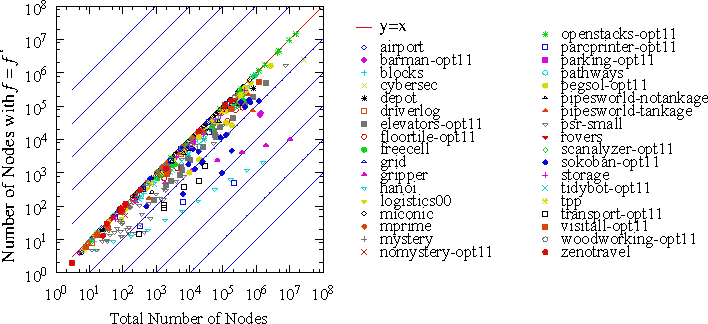
\includegraphics{tables/aaai16-frontier/aaai16prelim3/lmcut_frontier_noh-front.pdf}
 \caption{
 The number of nodes with $f=f^*$ (y-axis) compared to the
 total number of nodes in the search space (x-axis) with $f\leq f^*$ on 1104 IPC benchmark problems,
  using modified Fast Downward with \lmcut which 
  generates all nodes with cost $f^*$.
  }
 \label{fig:plateau-noh}
\end{figure}

This is visually described in \refig{fig:plateau-0}. Naively, the search space of \astar could be considered to have a thin layer of final plateau surrounding the closed nodes with $f<f^*$ (left), which is no longer true (as shown in \refig{fig:plateau-noh}). In reality, due to the curse of dimensionality, the search space has a large plateau of $f=f^*$ (right), and there is much room for improving the search within this region.

\begin{figure}[htbp]
  \centering
  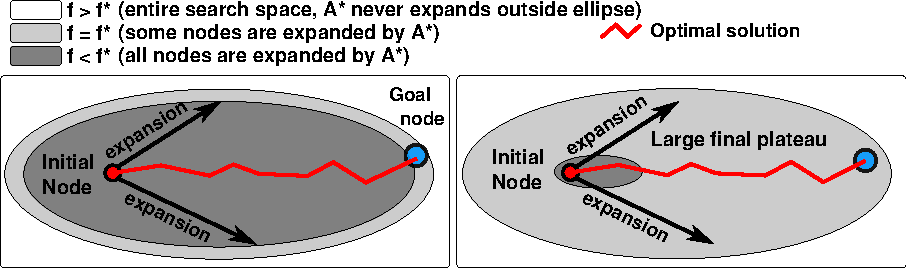
\includegraphics{img/astar/plateau-0.pdf}
 \caption{(Left) Naive and incorrect understanding of the search space. (Right) In reality, plateau containing the optimal goals ($f=f^*$) is large, and it even accounts for most of the search effort required by \astar.
  }
 \label{fig:plateau-0}
\end{figure}

Therefore, in those majority of IPC problem instances where the size of
the last layer ($f(n)=f^*$) of search is huge, a
\emph{tiebreaking strategy} can have a significant impact on the
performance of \astar. Tiebreaking strategy is a strategy 
for selecting which node to expand among nodes with the same $f$-cost.
It is widely believed that among nodes with the same $f$-cost,
ties should be broken according to $h(n)$, i.e.,
nodes with smaller $h$-values should be expanded first.  While this is a
useful rule of thumb in many domains, it turns out that tiebreaking
requires more careful consideration, particularly for problems where
this tiebreaking does not reduce the size of the plateau.

We empirically evaluate the existing, commonly used, standard
tiebreaking strategies for \astar (\refsec{sec:eval-common-strategies}).
We show that:

\begin{enumerate}
 \item Last-In-First-Out (\lifo) criterion tends to be more efficient
       than a First-In-First-Out (\fifo) criterion.
 \item Tiebreaking according to the heuristic value $h$, which
       frequently appears in the heuristic search literature, has little
       impact on the performance as long as a \lifo criterion is used.
 \item There are significant performance differences among tiebreaking strategies
       when domains include zero-cost actions. This is true even when
       both of the \lifo and $h$-based tiebreaking are enabled.
\end{enumerate}

While there are relatively few domains with zero-cost actions in the IPC
benchmark set, we argue that zero-cost actions naturally occur in
practical cost-minimization problems, and defines a new set of
benchmarks called \emph{zerocost domains}
(\refsec{sec:zerocost-domains}).  We empirically show that these
zerocost domains have the different search space structure and different
problem difficulty from those of the original domains.

In order to solve such problems more efficiently, we propose and
evaluate a new
tiebreaking method based on a notion of \emph{depth} within the plateau,
which corresponds to the number of steps from the ``entrance'' to
the plateau (\refsec{sec:depth},
\refsec{sec:depth-based-evaluation}). We also propose and evaluate an
admissible method which uses the distance-to-go estimate, an estimate which treats every actions
to have the unit costs (\refsec{sec:distance-to-go}).
In these sections, we empirically show that:
\begin{enumerate}
 \item Depth-based diversification strategy significantly improves the
       existing tiebreaking strategies using the same heuristic function.
 \item \emph{Inadmissible} distance-to-go variations of \emph{admissible} heuristics
       (\lmcut, \mands)
       significantly outperforms the tiebreaking using the original admissible heuristics.
 \item Distance-to-go variations of \emph{inadmissible} heuristics
       (\ff) further improves the performance by an order of magnitude.
 \item Distance-to-go variations of \emph{inadmissible} heuristics
       (\ff) combined with depth-based diversification further
       improves the performance.
\end{enumerate}

Finally, in \refsec{sec:discussion}, we discuss the implication by these
results. We offer a rather trivial, but new perspective to admissible
\astar search: \astar can be conceived as a sequence of independent runs
of satisficing Greedy Best First Search(GBFS)es in each plateau defined by the
$f$-value. We argue that arbitrary satisficing techniques improve the
search performance when applied as a tiebreaking strategy within
a plateau.
%  in the final plateau, which is the last and (usually) the largest
% layer of the search.
% 
Regressing from the new perspective, we also show a preliminary result
that the depth diversification tiebreaking, which has improved various
tiebreaking heuristics, also improves the performance of bare GBFS in
satisficing search.
We further discuss the future direction, related works, and close the article.

\textbf{
Note for reviewers:
This paper is a significantly extended version of the AAAI-16 paper by
the same authors. The addition to the conference paper is the following:
\begin{enumerate}
 \item Introduction of deterministic depth-based diversification
       strategy (as opposed to the randomized version in the conference
       paper), and its theoretical analysis in \refsec{sec:depth}. We
       also added thorough empirical analysis in
       \refsec{sec:depth-based-evaluation} that are not included in the
       conference version.
 \item Empirical analysis of distance-to-go estimates in
       \refsec{sec:distance-to-go}.  Also, we included an empirical
       evaluation of the use of inadmissible FF heuristics as part of
       tiebreaking criterion, and its combination with the
       depths metric thereof.
 \item New perspective to \astar and the preliminary results on the use
       of depth for satisficing planning (\refsec{sec:discussion}).
\end{enumerate}
}

